\section{Studie av konvektionsparametern}

Finita element har använts för att studera konvektionsparametern. Hastigeterna är alla
satta till noll på randerna med $h=6,19$ på de öppna randerna. Husets tak är adiabadiskt
och problemet är studerat under en natt i jämviktsläge (det vill säga en evig natt) med
$T_{ref} = \unit[0]{^\circ C}$ som referenstemperatur och $T_{inne} = \unit[20]{^\circ C}$ inomhus.
Väggens U-värde är satt till $U = \unit[1,18]{Wm^{-1}K^{-1}}$ vilket motsvarar söderväggen på fastigheten på Walleriusgatan.

\emph{\color{red} Behöver fyllas ut.}

\begin{figure}
\centering
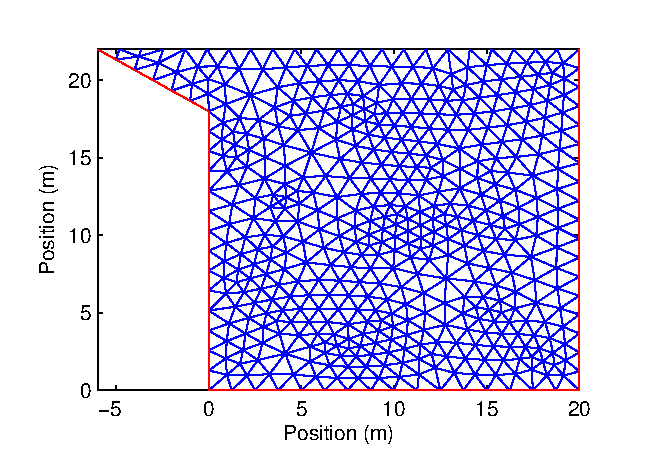
\includegraphics{images/triconvec.eps}
\caption{Definitionsmängd samt triangulering av problemuppställningen för studie av konvektion.}
\end{figure}
